\section{v1.0 补充实验与原始记录}\label{sec:legacy-experiments}
本附录保存 2026 年 11 月 20 日版本的实验。以下硬件线程数、运行总数和“全部实验”均指该历史协议；新增 ResNet-18 与矩阵分解结果采用正文中的 v1.1 协议。原始数值记录未因本轮增补而重写。
\subsection{公共协议与可重复性}
全部实验在 Windows 11、Intel Core Ultra 5 225H、约 32 GB 内存的本机上执行，采用 Python 3.12.14、NumPy 2.5.5 与 PyTorch 2.15.0+cpu。正式随机种子为 $0,1,2$，学习率选择种子为 42。原始记录保存每一步指标，汇总表给出三个种子的均值与样本标准差（分母为 $n-1$）。只有三个重复时，误差棒仅描述这三次运行的波动，不作总体显著性判断。

矩阵实验采用 NumPy float64，BLAS 固定单线程；语言模型采用 PyTorch float32，正式运行固定两个计算线程，并启用确定性算法。CPU 微基准分别记录 1、2、4 线程，正式实验始终使用统一的双线程设置。随机数据、初始化与训练批次分别由固定种子生成。计时使用单调高精度时钟，仍可能受操作系统调度与 CPU 频率影响。

本次包含 144 次确定性矩阵运行、48 次随机矩阵运行、108 条正交化配置测量、9 次语言模型试跑和 9 次正式语言模型训练。所有合成目标的权重衰减均为零。理论界用于期望量；把三个种子的实测平均画在理论界旁边是数值核对，不构成概率保证或数学证明。

\subsection{确定性矩阵二次问题}
构造
\begin{equation}\label{eq:synthetic}
 f(W)=\frac12\|A(W-W^\star)\|_F^2,
 \quad W\in\R^{32\times16},\quad A\in\R^{32\times32}.
\end{equation}
$A$ 的左右奇异向量由高斯矩阵 QR 分解产生，奇异值从 1 到 $\kappa^{-1/2}$ 按几何间隔排列。因此 $L=\op{A^\top A}=1$，Hessian 条件数恰为 $\kappa\in\{1,10,100\}$，目标下界为 0。初始位移归一化为 Frobenius 范数 1，各方法共享同一问题和初值。

比较梯度下降（步长 0.9）、EMA 动量梯度下降（$\beta=0.9$，步长 0.1），以及 $\beta=0$ 和 0.9 的精确 Muon。Muon 按 $\eta=0.1T^{-1/2}$ 设置步长，分别运行 $T=100,300,1000,3000$。基线步长是已知 $L=1$ 后的固定设置，不代表分别充分调参后的性能上限，也不用于声称公平的最优算法排名。

\begin{figure}[htbp]\centering
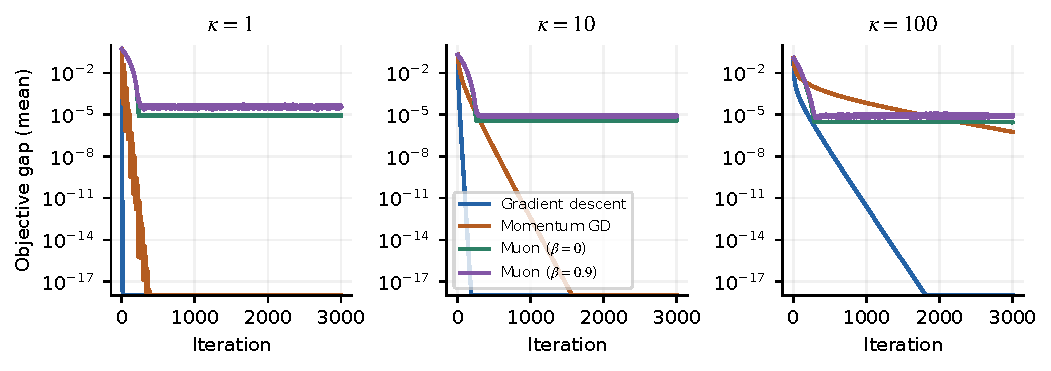
\includegraphics[width=\linewidth]{deterministic_loss.pdf}
\caption{确定性二次目标，$T=3000$。曲线为三个种子的目标差均值，绘图下限为 $10^{-18}$，因此底部截断不表示精确达到零。归一化更新与固定步长基线的运行方式不同，比较时需结合正文中的步长设置。}\label{fig:detloss}
\end{figure}

\begin{table}[htbp]\centering\small
\caption{$\kappa=10,T=3000$ 的确定性结果。末点目标差对应 $W_{T+1}$；平均梯度使用 $W_1,\ldots,W_T$。}
\begin{tabular}{lcc}\toprule
方法 & 末点目标差 & 平均梯度核范数 \\ \midrule
Gradient descent & $1.21\times10^{-32}\,\pm\,1.1\times10^{-33}$ & $0.002\,\pm\,0.000$ \\
Momentum GD & $1.79\times10^{-30}\,\pm\,7.6\times10^{-32}$ & $0.011\,\pm\,0.000$ \\
Muon ($\beta=0$) & $3.72\times10^{-6}\,\pm\,2.6\times10^{-7}$ & $0.046\,\pm\,0.002$ \\
Muon ($\beta=0.9$) & $7.56\times10^{-6}\,\pm\,9.9\times10^{-7}$ & $0.046\,\pm\,0.002$ \\
\bottomrule\end{tabular}

\label{tab:det}
\end{table}

梯度下降在低条件数二次问题上可以迅速降低目标值，说明这种问题并不是用来展示 Muon 全面优势的任务。Muon 的归一化方向在梯度变小后仍保留有限更新长度，因此常步长末段可能出现残差或振荡；动量也会使更新方向滞后于当前梯度。图\ref{fig:detrate}改变预算及相应步长，评价与定理一致的全程平均梯度，而非仅比较末点目标值。

\begin{figure}[htbp]\centering
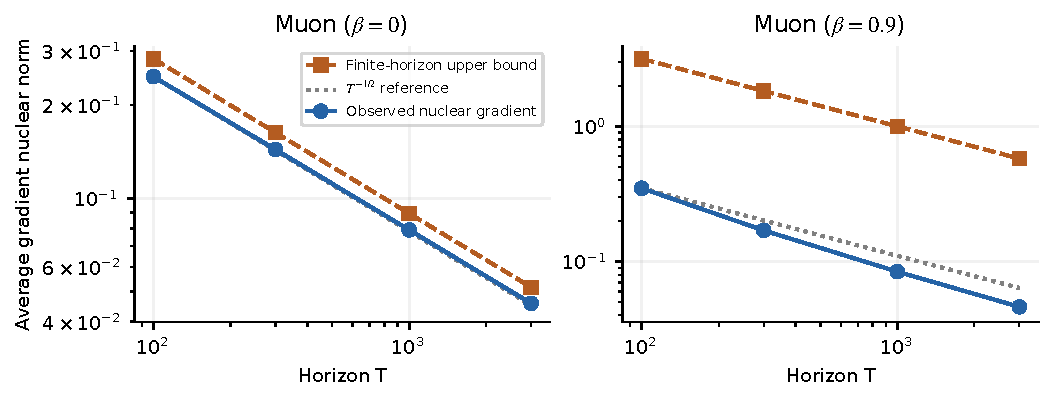
\includegraphics[width=\linewidth]{deterministic_rate.pdf}
\caption{$\kappa=10$ 下的预算实验。误差棒为样本标准差，虚线为显式有限步上界，点线仅为经过首个实测点的 $T^{-1/2}$ 参考线。}\label{fig:detrate}
\end{figure}

跟踪误差的通用估计使用了 $\sqrt r$ 与几何级数上界，因而非零动量下的理论常数可能相当保守。实验检查每一步式\eqref{eq:descent}，最大正向违反量为 \texttt{\MaxDescentViolation}，处于浮点舍入量级；这是实现与推导的一致性检查，不能替代前面的证明。

\subsection{已知方差的随机梯度问题}
固定 $\kappa=10$，使用
\begin{equation}\label{eq:oracle}
 G_t=\nabla f(W_t)+\frac{\sigma}{\sqrt{Bmn}}\Xi_t,
 \qquad (\Xi_t)_{ij}\overset{\mathrm{iid}}\sim\mathcal N(0,1).
\end{equation}
所以 $\E[G_t\mid\mathcal F_t]=H_t$ 且 $\E\|G_t-H_t\|_F^2=\sigma^2/B$。程序直接采样与 $B$ 个独立高斯噪声平均同分布的噪声，不实际计算 $B$ 次样本损失；因此这里只检验方差与梯度调用模型，不报告批量计算加速。

取 $\sigma\in\{0.01,0.1\}$、$B\in\{1,16\}$ 和 $T\in\{256,1024,4096,16384\}$，采用式\eqref{eq:schedule}及 $c=0.1$。每一步同时记录真实梯度、目标值和 $\|M_t-H_t\|_F$。真实梯度仅用于评价，优化更新只接触带噪声的 $G_t$。

\begin{figure}[htbp]\centering
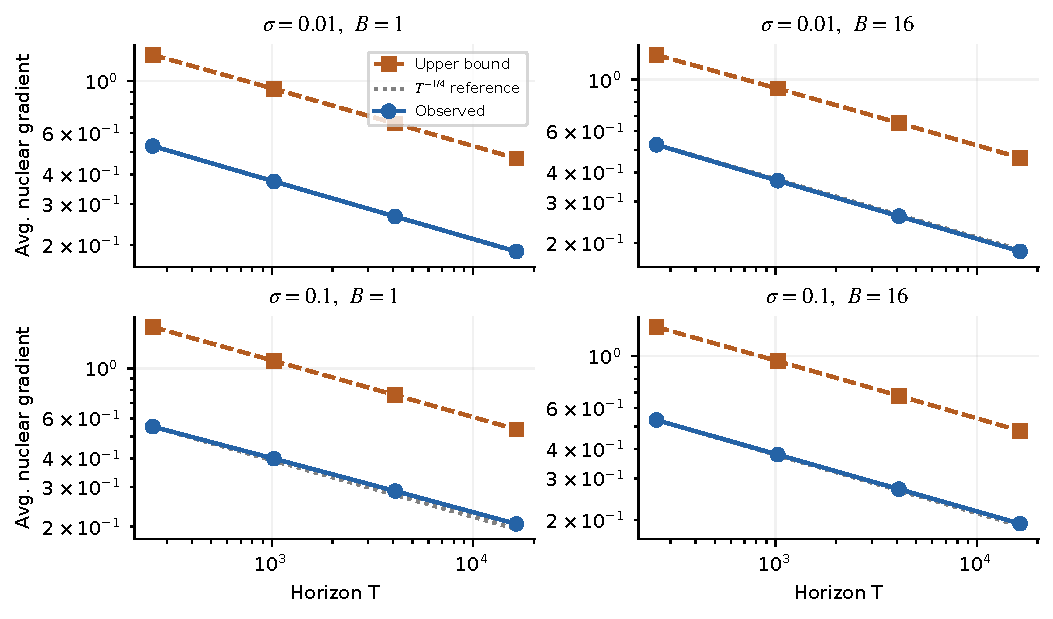
\includegraphics[width=0.96\linewidth]{stochastic_rate.pdf}
\caption{随机矩阵实验的全程平均梯度核范数。理论上界按同一问题的 $L,r,\Delta,\sigma,B$ 计算。灰色参考线没有进行曲线拟合。}\label{fig:stochastic}
\end{figure}

\begin{table}[htbp]\centering\small
\caption{$T=16384$ 的随机实验；全部数值为三个种子的均值与样本标准差。}
\begin{tabular}{ccccc}\toprule
$\sigma$ & $B$ & 平均梯度核范数 & 有限步界 & 平均跟踪误差 \\ \midrule
0.01 & 1 & $0.188\,\pm\,0.010$ & $0.468\,\pm\,0.010$ & $0.006\,\pm\,0.000$ \\
0.01 & 16 & $0.184\,\pm\,0.010$ & $0.462\,\pm\,0.010$ & $0.005\,\pm\,0.000$ \\
0.1 & 1 & $0.206\,\pm\,0.010$ & $0.537\,\pm\,0.010$ & $0.013\,\pm\,0.000$ \\
0.1 & 16 & $0.192\,\pm\,0.010$ & $0.480\,\pm\,0.010$ & $0.008\,\pm\,0.000$ \\
\bottomrule\end{tabular}

\label{tab:stochastic}
\end{table}

批量和噪声水平只改变误差分解中的随机部分，漂移部分仍由步长和动量共同决定。对这一强凸二次目标，实测下降可以快于一般非凸理论的最坏上界，也可能在有限预算中尚未进入渐近阶段。因此，图\ref{fig:stochastic}用于展示预算变化与界的保守程度，不把几个点的斜率当作收敛阶数的证明。全部精确 Muon 确定性和随机运行中，单次实测平均梯度与相应期望上界之比的最大值为 \MaxBoundRatio；随机样本不超界是本次结果，而非定理所要求的逐样本性质。

\subsection{有限步正交化的谱敏感性}
分别构造 $32\times32$、$64\times16$、$16\times64$ 矩阵。平坦谱的所有奇异值均为 1；病态谱从 1 到 $10^{-6}$ 按几何间隔排列；秩亏谱再把后一半奇异值置零。每个形状、谱和种子均测量 1、3、5、10 步 Newton--Schulz。精确极因子和多项式采用相同的紧致支撑约定。

\begin{figure}[htbp]\centering
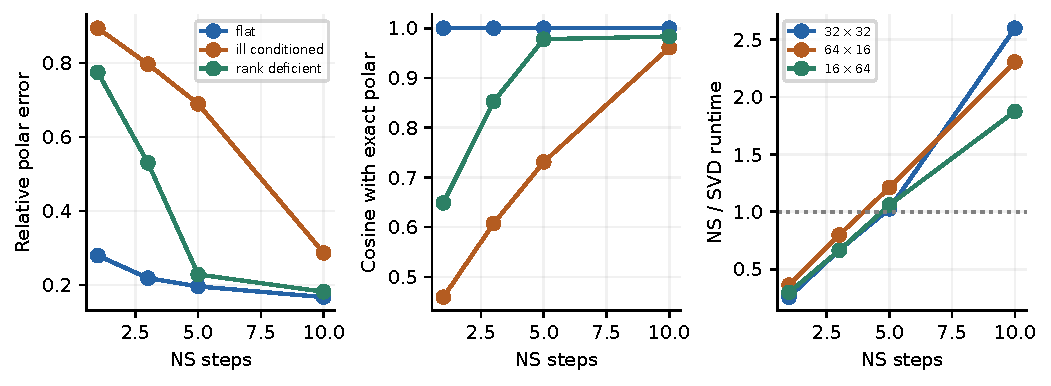
\includegraphics[width=\linewidth]{orthogonalization.pdf}
\caption{有限多项式的相对极因子误差、方向余弦和 CPU 耗时比。前两图跨形状与种子平均；右图跨谱与种子平均，每个计时重复 30 次。}\label{fig:ns}
\end{figure}

\begin{table}[htbp]\centering\small
\caption{五步 Newton--Schulz 与精确极因子的差异，跨三个形状和三个种子汇总。}
\begin{tabular}{lcc}\toprule
输入谱 & 相对 Frobenius 误差 & 方向余弦 \\ \midrule
平坦谱 & $0.197\,\pm\,0.133$ & $1.000\,\pm\,0.000$ \\
病态谱 & $0.690\,\pm\,0.003$ & $0.731\,\pm\,0.004$ \\
秩亏谱 & $0.229\,\pm\,0.009$ & $0.978\,\pm\,0.003$ \\
\bottomrule\end{tabular}

\end{table}

病态谱中的很小奇异值经过有限次多项式后仍可能远离 1，所以相对极因子误差与平坦谱明显不同。误差较大不等于该方向对目标必然无效：极因子误差对各支撑方向一视同仁，而真正的下降量是当前梯度与更新方向的内积。图\ref{fig:ns}同时报告方向余弦，以避免仅凭一个误差指标解释训练效果。此处矩阵尺寸很小、采用 CPU float64，计时比不能外推为 GPU 上大矩阵的性能结论。

\subsection{微型 Transformer 语言模型}
使用 Tiny Shakespeare\citep{karpathy2015}，词表包含 \VocabSize\ 个字符。按原始文本顺序划分后，训练、验证、测试集分别包含 \TrainChars、\ValChars、\TestChars\ 个字符，窗口严格限制在各自集合内。词表由整份公开语料的字符集合建立，只涉及字符编码，不用测试集选择模型或超参数。

模型为两层预归一化因果 Transformer\citep{vaswani2017}：宽度 64，4 个注意力头，前馈宽度 256，学习式位置嵌入，上下文 64，批量 16，不使用 dropout，不共享输入输出嵌入。参数总数为 \ParameterCount。两个 Muon 配置均只更新块内 8 个二维权重矩阵，其余参数使用 AdamW；全参数 AdamW 是基线。

先用种子 42 对每种配置分别试跑三个学习率，各训练 300 步，按末次验证交叉熵选取。AdamW 候选为 $\{0.0003,0.001,0.003\}$，Muon 候选为 $\{0.005,0.02,0.05\}$。辅助 AdamW 共享基线选出的学习率 \AdamLR。每种配置恰有三个候选，但这不是对不同优化器的穷尽搜索，也没有声称所有超参数都已最优。

\begin{table}[htbp]\centering\small
\caption{固定种子 42 的学习率试跑，选择依据仅为验证集交叉熵。}
\begin{tabular}{lcc}\toprule
方法 & 学习率 & 300 步验证交叉熵 \\ \midrule
AdamW & 0.0003 & 2.7250 \\
AdamW & 0.001 & 2.4640 \\
AdamW & 0.003 & 2.3875 \\
Muon-SVD+AdamW & 0.005 & 2.3506 \\
Muon-SVD+AdamW & 0.02 & 2.1306 \\
Muon-SVD+AdamW & 0.05 & 2.1332 \\
Muon-NS+AdamW & 0.005 & 2.3599 \\
Muon-NS+AdamW & 0.02 & 2.1497 \\
Muon-NS+AdamW & 0.05 & 2.1288 \\
\bottomrule\end{tabular}

\label{tab:pilot}
\end{table}

正式运行从头初始化，每次训练 1500 步，即处理 1536000 个训练字符目标。前 100 步线性预热，此后余弦下降到初始学习率的 0.1 倍。AdamW 使用 $(\beta_1,\beta_2)=(0.9,0.95)$、$\epsilon=10^{-8}$；Muon 使用 $\beta=0.95$ 和 Nesterov 修正。所有权重矩阵衰减系数为 0.01，偏置与归一化参数不衰减；不使用梯度裁剪。

每 50 步在固定 32 个验证批量上评价，选择验证损失最低的检查点，然后对完整测试划分计算一次交叉熵。测试窗口不重叠，相邻窗口共享一个作为上下文的边界字符，各目标字符除首字符外恰被评价一次。不同方法在相同种子下共享初始化和训练批次顺序。正式方法运行顺序随种子轮换，减少固定顺序对计时的影响。

\begin{figure}[H]\centering
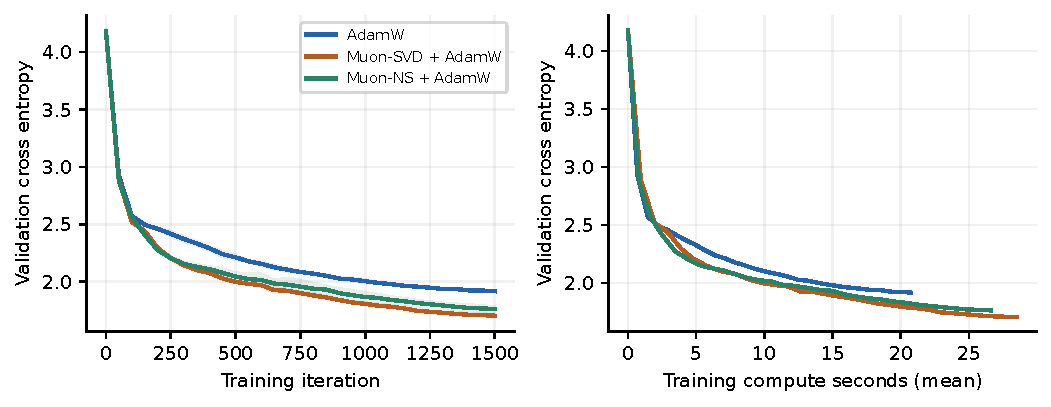
\includegraphics[width=\linewidth]{language_learning.pdf}
\caption{语言模型验证曲线。左图阴影为三个种子的样本标准差；右图把同一步的平均验证损失放在平均训练计算耗时处，并非对相同墙钟时刻插值。训练计算耗时包含采样、前后向传播和更新，不包含验证、测试、数据下载及检查点写入。}\label{fig:lm}
\end{figure}

\begin{table}[H]\centering\small
\caption{微型语言模型正式结果。测试指标来自按验证集选择的检查点；困惑度为 $\exp(\mathrm{CE})$，先对每个种子计算，再汇总。}
\resizebox{\linewidth}{!}{\begin{tabular}{lcccc}\toprule
方法 & 学习率 & 测试交叉熵 & 测试困惑度 & 训练计算耗时 / 秒 \\ \midrule
AdamW & 0.003 & $1.962\,\pm\,0.007$ & $7.110\,\pm\,0.047$ & $20.710\,\pm\,1.841$ \\
Muon-SVD+AdamW & 0.02 & $1.793\,\pm\,0.008$ & $6.008\,\pm\,0.051$ & $28.504\,\pm\,0.781$ \\
Muon-NS+AdamW & 0.05 & $1.843\,\pm\,0.025$ & $6.316\,\pm\,0.156$ & $26.577\,\pm\,0.563$ \\
\bottomrule\end{tabular}
}\label{tab:lm}
\end{table}

本次 AdamW、Muon-SVD+AdamW 与 Muon-NS+AdamW 的测试交叉熵均值依次为 \AdamCE、\SVDCE、\NSCE，训练计算耗时均值依次为 \AdamTime、\SVDTime、\NSTime\ 秒。表\ref{tab:lm}与图\ref{fig:lm}需要同时阅读：较低的按步数损失并不自动对应较少的计算时间。精确 SVD 对照用于隔离正交化方式，其计算代价本来就可能高于有限矩阵多项式。

三种配置共同改变了训练轨迹，混合 Muon 与全参数 AdamW 的比较不能单独识别某个参数组的因果贡献。小字符模型、短上下文、有限训练预算和三个种子也限制了结论范围。这里报告实际测量，不把未达到的固定损失阈值换算为假想加速比，也不把优化过程的定理直接解释为泛化保证。
\FloatBarrier
